\chapter{Problemanalyse}\label{ch:analyse}
\section{Vigtighed af administration og IT i virksomheder}
Hvad vil dette afsnit?\\
- opstille fakta\\
    - Administration af virksomheder\\
    - reelle og aktuelle problemer\\
    - skal være i forhold til det initierende problem


Dette afsnit vil belyse en række egenskaber som IT administration medfører. Dette inkluderer fordele og ulemper ved IT systemer samt virksomhedernes nødvendighed i at holde sig konkurrencedygtige. Afsnittet underbygger den initierende problemstilling og undersøger de eksisterende positive og negative sider af IT administration. Dette opnås ved at undersøge en række kilder for relevant data om IT administrations effekt på arbejdsmiljøet og konkurrencedygtigheden.

\subsection{IT administration}
Det bliver vigtigere for virksomheder at benytte IT redskaber til administrativt arbejde og til at få virksomhedens daglige rutine til at fungere. Uden IT falder virksomheder konkurrencemæssigt bagud, da de ikke er i stand til at udfører opgaver lige så effektivt som deres konkurrenter. Væsentligheden af IT beskrives således af IBiz Center: \textit{"IT-integration er alfa og omega"} \citep{case_green_team}. Desuden kan IT systemer bruges til at løse en række forskellige administrative opgaver på en gang. Færre processer gør, at det bliver nemmere for ledelsen at udføre dem \citep{Ibiz_streamline}. Ved brug af IT systemer, i stedet for manuelt eller på papir, kan integriteten af tal og informationen desuden sikres. Således sikres personalet ikke at få for lidt i løn, kunder får de rigtige varer og tjenester og varer ligger de angivne placeringer i lageret osv. \citep{Ibiz_streamline}. Ved at benytte et system, der undersøger om dataen er korrekt, kan virksomheden både spare tid og penge \citep{case_green_team}. 

\subsubsection{Cloud computing}
Uanset hvilken sektor og branche en virksomhed befinder sig i, sker der en stigning i brug af IT som set på figur \ref{fig:virksomcc}. Figuren viser stigningen af \textit{"Virksomheder der anvender cloud computing"} fra år 2012 til 2014. Selvom cloud computing ikke er den eneste form for IT løsning til virksomheder, står den for over en tredjedel af de anvendte IT løsningerne, og er dermed ikke ubetydelig. Derfor kan vi uddrage vigtige information om IT-brug fra Dansk Statistik data om cloud computing \citep{itvirk}.\todo{Hvilken information er det vi kan uddrage og hvad bruger vi den til?}

\begin{figure}[H]
    \centering
    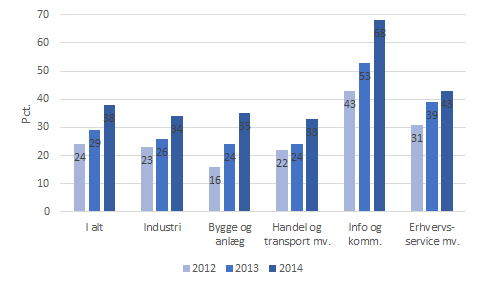
\includegraphics[width=1\textwidth]{figures/CloudComputingStatestik.png}
    \caption{Statistik over virksomheder, som benytter cloud computing \citep{itvirk}.} 
    \label{fig:virksomcc}
\end{figure}

\begin{figure}[H]
    \centering
    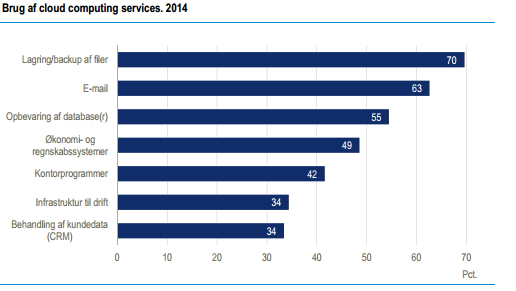
\includegraphics[width=1\textwidth]{figures/brugafccservices.png}
    \caption{Statistik over distribution af Cloud Computing brug \citep{itvirk}}
    \label{fig:distcc}
\end{figure}

%\newpage
På figur \ref{fig:distcc} ses det, at over halvdelen af virksomhederne, som anvender cloud computing, bruger løsning til opgaver som filhåndtering og database brug, samt e-mail. Dette tager næsten to tredjedele af al cloud computing brug i virksomheder\todo{Jeg er ikke helt sikker på hvad de næsten to tredejedel er? kan du bruge lidt flere præcise tal til at forklare det. Hellere tal end et skøn}. Yderligere vises det at over en tredjedel benytter det til infrastruktur, kundedata, økonomi mm. Cloud computing mindsker også mængden af tid der bruges på vedligeholdelse af systemet da udbyderen af cloudcomputing er ansvarlig for vedligeholdelsen. 

% Luca skrive hvilke konsekvenser der følger med denne løsning. 
Cloud computing har den fordel, at det er allestedsnærværende. Uanset hvor en medarbejder befinder sig, enten på arbejde eller derhjemme, er der mulighed for at arbejde. I toget, derhjemme eller til møde, det er altid muligt at tilgå sine dokumenter, e-mails, applikationer, osv. Flere virksomheder benytter dette, så deres medarbejderne bruge mere energi på deres arbejde, fordi at man altid har arbejdet med sig, da pc, tablet, smarthphones, osv. gør at man altid mulighed for at tilgå det. Der er altså tale om textit{"det grænseløse arbejde"} \citep{SystimeStress}, da man nu har mulighed for at tage arbejde med hjem. Det grænseløse arbejde, er blevet mere udbredt i forbindelse med samfundets udvikling, fordi der sker en stigning af folk med karrierelivsformen samt teknologien gør det lettere at have denne livsform. At være fleksible er derfor blevet en præmis indenfor arbejdsmarkedet. Denne udvikling giver det fleksible menneske flere muligheder i form af jobs og uddannelse, men medfølger at arbejdslivet er blevet mere uforudselig, hvilket kan være stressende. Fleksibilitet kan altså have en stressende effekt på arbejdslivet, det er derfor vigtig at tage hensyn når vi implementere en løsning, men dette kan være svært ud fra et datalogisk synspunkt, da det er mere et identisk følge af benyttelsen af ny teknologi, frem for teknologien selv. \citep{SystimeStress} 

Dog skal det bemærkes at cloud computing ikke er en perfekt løsning. Dropbox, en cloud storage service, er et eksempel. På deres hjemmeside står der, at de stræber efter \textit{"100\% uptime"} men at \textit{"det er urealistisk at garentere det"} \citep{drpbx_downtime}. Ved brug af cloud computing er det vigtigt at være opmærksom på den downtime servicen el.lign. har. Nogle services kan f.eks. have downtime i løbet af ugen, hvis de skal vedligeholde deres udstyr.

IT Administration er som regel Enterprise computing ->
Cloud Computing pga. naturlig udvikling (SaaS). 
Cloud computing for os, hvis vi har tid.
Cost savings (side 4)


Cloud

Når nye IT systemer bliver implementeret er det vigtigt at der er styr på at de fungerer korrekt. Der er tilfælde hvor nye IT systemer ikke har fungeret optimalt. Dette kan observeres ved systemer som fx ”amanda” eller ”EFI” som kostede staten over 1 milliard kroner, uden at blive sat i brug \citep{DrItsys}. \todo{Syntes det virker lidt hurtigt skrevet og meget kort -- Er det her faktisk relevnt for denne section?} I takt med at mindre virksomheder udvider, samt den konkurrence imellem virksomheder, er der stigende krav til kvantiviteten og tempoet hos administrationen i virksomhederne. Denne ekstra belastning kan resultere i dårlige arbejdsforhold, hvilket vil sænke produktiviteten yderligere. Et IT-værktøj til at afhjælpe i administrations delen ville kunne lette en sådan belastning og dermed forbedre arbejdsmiljøet \citep{It_armil}. 

%\section{Hvorfor mindre virksomheder ikke udvider}
%Der eksisterer en del mindre virksomheder indenfor byggebranchen, mange af dem vælger ikke at blive større, når håndværkermesteren indtjener det han gerne vil. Udover det virker administrationen for mange af de små virksomheder som uoverskuelig. De vælger ikke at udvide pga. manglende overskuelighed med hensyn til administration. Flere af dem frygter at miste overblikket over deres administration, hvis de udvider deres virksomhed og ansætter flere. I stedet vælger de at beholde deres størrelse, som en virksomhed på én til fire personer %\citep{SmaaFirmaerOrker}.
%I 2012 blev der indført en ny lov, som skræmte små virksomheder yderligere fra at udvide. Denne lov ville give virksomheder, som ikke havde administrationen i orden, bøder.\todo{Skal der bare stå bøder eller skal det omformuleres?} Denne lov rammer især de små virksomheder %\citep{Nyeadmboder}.
%Et eksempel på en type virksomhed, som ikke udvider, er håndværkervirksomheder. Tre ud af fire af disse virksomheder har kun én til fire ansatte. Dette skyldes som nævnt før, at de frygter administrationen af flere ansatte end dem de allerede har. De fleste af disse virksomheder er ofte ejet af en dygtig håndværker, hvor administration ikke er en del af personens %kompetencer \citep{SmaaFirmaerOrker}. \todo{Afsnittet skal generelt kigges på}


\section{Arbejdsmiljø}
\noindent Mangel på IT administration kan have negativ påvirkning på en arbejdsplads, og skabe et ineffektivt arbejdsmiljø. Videncenter for arbejdsmiljø har lavet en definition på begrebet arbejdsmiljø som lyder således: \textit{"Arbejdsmiljø er et samspil af de relationer, påvirkninger og vilkår, som mennesket arbejder under. Det er også den tekniske og sociale udvikling af arbejdspladsen, som kan bidrage til det enkelte menneskes sikkerhed på kort sigt samt til menneskets fysiske og psykiske sundhed på længere sigt"} \citep{Arbejdsmiljoe}.

Et arbejdsmiljø kan have mange forskellige påvirkninger på arbejderen. Eksempler på disse kan være: 
\begin{itemize}
    \item {\textbf{Psykisk påvirkning} \citep{Arbejdsmiljoe_psykisk}}
    \begin{itemize}
    \item {\textbf{Stress}: At arbejde kan være stressende, og dette kan have indvirkning på både arbejderen og arbejdsmiljøet. Stress kan f.eks. give hukommelsesbesvær, koncentrationsbesvær og nedsat humør. Disse faktorer kan både påvirke arbejderens arbejdsproces og arbejderens arbejdsomgivelser \citep{Arbejdsmiljoe_stress}.}
    \end{itemize}
    \item {\textbf{Fysisk påvirkning} \citep{Arbejdsmiljoe_fysisk}}
    \begin{itemize}
    \item {\textbf{Slid}: Et arbejde kan være fysiskt hårdt på mange måder. Dårlige muse anordninger til computerbrug kan f.eks. resultere i skader i håndled \citep{Arbejdsmiljoe_fysisk}.}
    \item {\textbf{Støj}: En larmende arbejdsplads kan også have stor indvirkning på arbejderens hørelse, i form af fysiske høreskader og er også en faktor til psykisk stress \citep{Arbejdsmiljoe_stoej}.}
    \item {\textbf{Klima}: Aspekter som for høj eller for lav temperatur (højere end 25 grader, lavere end 20 grader), og et indelukket eller forurenet klima, kan have fysisk påvirkning på medarbejderen i form af f.eks. tørre øjne, træthed og hovedpine \citep{Arbejdsmiljoe_indeklima}.}\\
    \end{itemize}
\end{itemize}

Med henblik på IT administration, kan den negative påvirkning forekomme, når der er en mangel på effektiv IT administration, som f.eks. over-krævende- og uflexible arbejdsplaner, hvilket kan resultere i stress hos den enkelte medarbejder\citep{Cambridge2011}.

\subsection{Vagtplanens indflydelse på arbejdsmiljø}
For at forebygge konsekvenserne af et dårligt arbejdsmiljø, er en struktureret eller fleksibel vagtplan en mulighed. En fleksibel vagtplan, hvor medarbejderen er med til at vælge sine vagter, vil udover at skabe en større medarbejdertilfredshed også ansvarliggøre den enkelte medarbejder. En fleksibel vagtplan vil sikre et bedre arbejdsmiljø, ved at skabe større fleksibilitet mellem arbejde og privatliv. Det øgede ansvar giver også medarbejderen en forståelse for arbejdsplanlægningen og skaber dermed et større engagement, i at få arbejdsplanen til at gå op. Samtidig vil vagtplanlæggeren få mere tid til andet arbejde som f.eks. kvalitetssikring.
Undersøgelser viser også, at gode og fleksible arbejdstider er fastholdelses potentiale for medarbejderne, hvilket vil sige at kontinuiteten opretholdes. \\

\subsection{Fleksibel arbejdstid}
\noindent Dette afsnit tager udgangspunkt i artiklen: \textit{Ny fleksibel arbejdstid gav mere arbejdsglæde} \citep{Thomse2014}. På et plejehjem\todo{Lyder det ikke lidt sjovt at starte på den måde?-Smed} blev der implementeret et IT-system, hvor medarbejderne selv skulle vælge sine vagter. Ifølge artiklen blev IT-systemet indført fordi \textit{"at man gerne vil forebygge overbelastning af de stadig færre, der vælger at arbejde i sektoren og dermed også både fastholde dem i jobbet og rekruttere nye."} IT-systemet har givet medarbejderne mere frihed, da muligheden for selv at vælge vagter, gør det lettere at tilpasse sig. Systemet virker ved at medarbejderne starter i en ønske fase, hvor de vælger de tider og dage de helst vil arbejde. Herefter bliver ønskerne puslet sammen i fællesskab, sådan at der altid er et tilstrækkeligt antal medarbejdere på arbejdet. Plejehjemmet udmelder at i denne sammenhæng, kan det være fornuftigt at have en blanding af medarbejdere der har, og ikke har børn. Der kan altså uddrages at på en arbejdsplads som et plejehjem, hvor der skal være folk på arbejde hele tiden, at det er en fordel for medarbejderene at have indflydelse på hvilke tidspunkt de gerne vil arbejde, da det kan være en smule anderledes i forhold til en normal arbejdsplads, med faste arbejdstider. Derfor kan det være med fordeling af arbejdet, hvis man har forskellig kategorier af mennesker. Folk med børn kan have det bedre med normal tider, så det passer med skole, fritid, osv. hvor at medarbejder uden børn har letter ved at tage de lidt mere atypisk vagter, som i weekenden eller om natten. Der er altså tale om en kategorisering af medarbejder. Denne fleksible IT løsning reducerer også de mistænkelige sygedage (dage hvor folks sygedom betvivles), fordi at medarbejderne selv fik mulighed for at vælge, hvilke dage de ville have fri. Den generelle stemning på arbejdspladsen er også blevet væsentligt bedre, da medarbejderne selv har valgt deres vagter, hvilket gør det svært at være utilfreds med arbejdstiderne. 
IT-systemet har derimod ikke kun været godt. I starten forholde nogle af medarbejderne sig konservativt til løsningen og var tilfredse med vagtsystemet som de havde før. Efterhånden begyndte næsten alle dog at kunne se fordelene ved det nye IT-system.

\section{Interessentanalyse}
I dette afsnit undersøges de parter som har interesse i arbejdsplanlægning. Dette gøres gennem analyse af interessentens fokusområder på problemet samt hvilke krav de har til en eventuel løsning af problemet.

Med henblik på et givet problem, vil der være interessenter, der er interesserede i en løsning til det givne problem. Herved bliver interessentanalysen brugt til at finde de interessenter, der er interesserede i at løse problemer angående ineffektiv administration og IT i små virksomheder, med henblik på planlægning.
Derfor er denne analysemodel nyttig til at identificere de vigtigste interessenter, sådan at der tages forbehold for interessenternes ønsker og eventuelle parter, som kunne ønske at have en negativ indflydelse på problemet. Efter at interessenterne er identificeret gennem brainstorming, bliver de placeret i en Påvirkning og Indflydelse Matrix \ref{fig:PavirkInflydMat}, som opdeler interessenterne i fire kategorier. Herefter bliver interessenterne opdelt i prioriteret rækkefølge med henblik på vigtighed for problemløsningen.

\subsection{Medarbejder} Sekundær
Medarbejdere er interesseret i en løsning på problemet grundet, at de kommer til at benytte løsningen i forbindelse med deres arbejde. Deres samarbejde er vigtig for gennemførelsen af løsningen, da implementeringen afhænger af medarbejdernes samarbejdsvillighed. Selvom deres deltagelse er vigtig, har de ikke nogen indflydelse på løsningens udformning, da det oftest vil være en chef, som står for arbejdsplanlægningen og dermed bruger de blot den gennemarbejdede arbejdsplan. Medarbejdernes holdninger til projektet kan variere alt efter hvilken erfaring de har med det nuværende system. Det kan f.eks. være problematisk at skulle sættes ind i et nyt system, hvis de lige har lært at bruge det nuværende. Dog kan det også være at løsningen tilvejebringer en bedre måde for dem at håndtere deres arbejdsplan, hvorved de får mere overblik over deres arbejdstider. Medarbejderne er sat ind i figur \ref{fig:PavirkInflydMat} som gidsler. De er sat der fordi at deres medvirken er vigtig for problemløsningen, idet at det er dem der skal bruge den, men ikke har nogen påvirkning på løsningen af problemet.\todo{kilde}

\subsection{Leder} Primær
Lederen kunne være interesseret i et struktureret skema, da det primært er dem som holder overblik over medarbejderne og sørger for at de kommer til tiden. Derfor er lederen også vigtig for udviklingsprocessen, da det er dem som har erfaring indenfor planlægning og kender behovene indenfor for dette. I udviklingprocessen er det også lederen der skal forklare de krav og de behov som arbejdsplanlægningen, for den virksomhed som vedkommende leder, har brug for. Bedre struktur kan også gøre det muligt for lederen at holde styr på hvor meget den individuelle medarbejder arbejder, sådan at reglerne om arbejdstid overholdes.
Ifølge artiklen "4 trin til planlægning der holder", er lederen en interesseret i effektive planlægnings værktøjer, fordi at disse giver lederen et større overblik og bedre fokus hvilket gør lederen mere effektiv \citep{Kolding2012}. Lederen er en ressourceperson \ref{fig:PavirkInflydMat}, fordi at lederen både har en påvirkning på problemløsningen,  og fordi hans medvirken er vigtig for at løsningen kan blive en succes, idet at det er ham der har styr på hvad en god arbejdsplanlægningsløsning skal indholde.

\subsection{IT-leverandør}
IT-leverandøren er det firma som sælger eller eksporterer IT-hardware til en virksomhed. De sælger produkter som computere, telefoner eller lignende, som hjælper virksomheden med administration.
IT-leverandøren, har ikke stor indflydelse på løsningen og har heller ikke en vigtig medvirken i gennemførelsen af løsningen. De sørger dog for udstyr som kan bruges af virksomheden efter produktet er blevet udviklet. Pga. førnævnte så er er IT-leverandøren sat som Ekstern \ref{fig:PavirkInflydMat}.\todo{kilde}

\subsection{Kunde}
Kunderne for firmaet er også en interessent, da de modtager den service som firmaet tilbyder og er derfor direkte påvirkede af firmaets effektivitet. Lange køer kan f.eks. have stor indflydelse på kunden, idet at kunden skal bruge længere tid i f.eks. et supermarked, end kunden skulle gøre hvis der ikke var nogen kø \citep{Brix2012}. Sådan et problem ville kunne løses med ordentlig arbejdsplanlægning, der satte nok medarbejdere de rigtige steder i supermarkedet, for at skabe en hurtig kundeekspedition. Kunderne er brugere af firmaet, men de har ikke nogen indflydelse eller medvirken på problemløsningen. De bliver indirekte påvirket af løsningen, hvilket er grunden til at de ikke har nogen indflydelse på udformningen af løsningen. Kunderne er derfor sat som Ekstern \ref{fig:PavirkInflydMat}.

\subsection{Staten} Tertiær
Staten har en interesse i at sikre et god arbejdsmiljø i Danmark. De er interesserede i at mindske stress på arbejdsmarkedet samt sikre et godt arbejdsmiljø. Et eksempel er deres kampagne \textit{"Fra stress til trivsel"} som viser statens interesses i at mindske stress på arbejdsmarkedet \citep{Arbejdsmiljoe_Arbejdspladser}. Statens kampanger tilbyder arbejdspladserne materiale og ressourcer til løsning af eventuelle stress relaterede problemer men arbejdspladsen selv skal stå for at udnytte ressourcerne. Staten har derved ikke interesseret i selv at skulle reagerer på hvert eneste arbejdsplads. Derfor har de ikke stor indflydelse eller medvirken i løsningen af problemet da den individuelle arbejdsplads selv skal gøre brug af kampagnen. Beskæftigelsesministeriet er en del af staten og er dette ministerium opgave at fremlægge lovforslag til arbejdsmiljøloven samt at sikre at lovene bliver opretholdt \citep{Beskaeftigelsesministeriet2002}.

\subsubsection{Arbejdstilsynet} Tertiær
Arbejdstilsynet er en del af Beskæftigelsesministeriet og har til opgave at sikre et bedre arbejdsmiljø i Danmark. Arbejdstilsynet er nedsat til at sikre at arbejdsforholdene på de danske virksomhederne er sikkerheds- og sundhedsmæssigt fuldt forsvarlige på baggrund af arbejdsmiljøloven. Dette gøres ved at arbejdstilsynet fører tilsyn med virksomhederne og derved sikre at arbejdsmiljøloven bliver holdt \citep{Arbejdstilsynet2015}. Arbejdstilsynet er derfor interesserede i dårlig arbejdsmiljø som fælge af dårlig arbejdsplanlægning, da lovgivningen nedsætter de gældende regler for arbejdstid og hviletid. Virksomhederne er derfor nød til at lave deres vagtplaner med baggrund i lovene om arbejdstid. På den måde står staten og arbejdstilsynet som en grå eminence \ref{fig:PavirkInflydMat}, da de fastsætter og håndhæver en række love som har indflydelse på problemet men som samtidig ikke har stor medvirken i løsningen af problemet \citep{Beskaeftigelsesministeriet2002}.

\subsection{Prioriteringen af interessenter}
Ud af de seks førnævnte interessenter, så udvælges de vigtigste med henblik på en problemløsning i forhold til arbejdsmiljø, menes at være vigtigere end de andre. Disse interessenter bliver så sat i prioriteret rækkefølge som henholdsvis primære, sekundære og tertiære interessenter. Lederen blev udvalgt som den primære interessent idet at det er dem der styrer virksomheden med hensyn til vagtplanlægning, så en given løsning ville påvirke og gavne dem mest. Medarbejderen blev udvalgt som sekundær interessent fordi at de har så meget indflydelse på styringen af virksomheden som lederen har. De har derfor ikke nogen indflydelse på hvilken vagtplanlægningsløsning der bliver brugt, dog er de brugere af den, og ønsker derved en optimal løsning.
Staten blev udvalgt som en tertiær interessent fordi at de kun har en påvirkning på en problemløsning. De har kun indirekte medvirken i problemløsningen, og er der kun til at skabe samfundsmæssige retningslinjer for problemløsningen. 


\subsection{Interessekonflikter}


\section{Interview}
Det kvalitative forskningsinterview forsøger at forstå verden fra informantens synspunkt, herunder meninger og holdninger. Viden i forskningsinterviewet skabes i interaktionen mellem interviewer og informant. Interview er valgt frem for et spørgeskema, da den viden intervieweren får ved et interview, ikke nødvendigvis ville opstå i en spørgeskemaundersøgelse. Interview giver informanten mulighed for at fordybe sig i og udforske egne oplevelser og meninger. Den viden der opnås ved et interview, er socialt konstrueret, da det ikke bare er en dataindsamling, men at der skabes data gennem den førnævnte interaktion \citep{kvale2009}.

Ved hjælp af interessentanalysen, er det blevet klargjort, hvilke personer der kunne være interesserede i en løsning. Ved interviewene stræbes der efter at opnå en viden omkring hvilke problemer der er ved nuværende løsninger, samt krav til fremtidige løsninger. Interviewet blev herefter brugt til at skabe indsigt indenfor emnet. Spørgsmålene blev lavet på baggrund af nogle emner der skulle belyses. Udfra disse emner, blev nogle korte og åbne spørgsmål lavet, for at sikre, at den viden der opstod blev reflekteret over. Dette ville ikke være muligt med f.eks. ledende spørgsmål, hvor informanten bliver påvirket i en bestemt retning. Ved hjælp af svarene fra interviewene blev det gjort klart, hvilke problemer der var med de nuværende systemer, samt positive sider heraf. Udfra disse data kunne en foreløbig kravspecifikation dannes.
\\

\subsection{Analyse af interviews}
De seks interviews blev foretaget i seks forskellige butikker for at sikre diversitet blandt informanternes svar. Dette gav også flere systemer at få respons på. 
\\Hos Home blev der brugt ikke brugt et system som sådan, men bare en fast kalender. Dette kunne være fordi, at de ikke var særligt mange på arbejde, samt at de var fuldtidsansatte. Dette giver ikke et behov for en fleksibel arbejdsplan, men i stedet en struktureret. Dog blev der her kørt med tre ugers vagtplaner, hvilket giver en smule fleksibilitet. Processen med at få lavet en vagtplan bliver beskrevet således: ”Der bliver lavet i en manuel kalender først, så bliver det bare proppet ind i kalenderen deroppe.” Dette kunne tyde på, at det er en simpel proces. Dette kan igen hænge sammen med, at de ikke var særligt mange samt at de var fuldtidsansatte. Fuldtidsansatte arbejder 37 timer i ugen, og dermed er der ikke det store behov, for at skulle ændre på vagtplanen, da ingen rigtigt har nogle fridage. Denne metode står i kontrast til interviewene med KIWI, Rema 1000, Netto og Friluftsland. Her står Friluftsland ud, da de tre førstnævnte alle går ind under kategorien, dagligvarebutikker, mens Friluftsland mere en specialforretning. Friluftsland bruger et system der hedder Staffweb. Her bliver står butikschefen at lave vagtplanen inde i programmet. Så kan medarbejderne selv tilgå vagtplanen via programmet, hvilket minder om Homes løsning, som kunne tilgå vagtplanen via deres kalender. Staffweb tilbyder dog også flere features. Der bliver f.eks. lagt stor vægt på, at der skabes et overblik over butikken og sine medarbejdere i Staffweb. Her er taxerne for de forskellige dage samt de forskellige medarbejdere lagt ind, sådan at der hele tiden er et godt overblik over lønbudgettet. Udover det, så kan chefen også se, hvor tit en person bytter sine vagter eller tager ledige vagter. Ved bytning af vagter, bliver vagterne lagt op i en bytte-børs. Dog skal medarbejder stadig igennem chefen for at gøre dette. Der bliver også tjekket op på, om medarbejderne møder ind til tiden, da de skal stemple ind når de møder. Igen giver dette et godt overblik. KIWI benytter sig af samme system som Friluftsland. Som det bliver beskrevet i interviewet med KIWI, så fungerer dette system bedre end det tidligere papirformssystem; “I forhold til før hvor vi havde det på papiret, der er det nemmere, fordi enhver har ikke undskyldningen med, min vagtplan er blevet væk, fordi man kan altid bare gå ind på nettet, også trykke, og for det er en simpel kode og et simpelt brugernavn som er bestemt af firmaet, så man kan altid finde det, så det er en klar fordel i forhold papir vagtplaner, bare det at det ikke kan blive væk, man har aldrig undskyldning, det vidste jeg ikke.” Da disse butikker har deltidsansatte skaber dette et behov for en fleksibel vagtplan, og ud fra ovenstående citat, kan det uddrages, at dette system hjælper på dette. Da der er flere deltidsansatte hos KIWI, gør dette også, at vagtbytning ofte hænder. Dette sker ved, at chefen bliver kontaktet, sådan at vedkommende er klar over, at en vagt er blevet byttet; “Vi vil have det på sms, sådan så at vi kan sige, du skrev til mig og det er sådan det er, så kan vi altid have det.” Ligesom i Friluftsland skal medarbejderne igennem chefen, for at kunne bytte vagter.
En mangel ved Staffweb bliver i KIWI beskrevet således: “Systemet mangler den ting, at når en medarbejder stopper, at man så kan fortsætte vagtplanen i en anden persons navn, du kan ikke bare rykke, sige alle den persons vagter, skal flyttes over til den person.” Dette kunne igen tyde på et behov hos virksomheder med deltidsansatte eller flexarbejdere.
I Netto bliver Teamplan brugt. Teamplan giver også god overblik omkring økonomi, hvilket gør at chefen igen ikke skal gøre det store arbejde med den del: “Det regner lønnen ud også. Hvor meget man lægger til at bruge om måneden på året og på ugen og på dagen, alt. Og selv for at man får helligdagstillæg aftentillæg jeg skal ikke ligge noget som helst ind. Det er systemet selv sat op til jeg kan ikke gøre noget forkert så længe medarbejderen scanner når det kommer og går.” Dette giver et ansvar til medarbejderen om at få stemplet ind. En afvigelse fra KIWI’s og Friluftslands løsning er måden at bytte vagter på. Hvor de ved KIWI og Friluftsland skulle igennem chefen for at få lov at bytte vagter, så sker det hele internt hos Netto. Dette giver endnu mere ansvar til medarbejderen, hvor der bliver lagt stor vægt på tilliden mellem medarbejder og chef.
Den sidste dagligvarebutik, Rema 1000, bruger et helt tredje system, Tamigo. En fordel ved dette bliver beskrevet således: “Det er overskueligt, det er funktionelt vedrørende både med telefonnumre, oplysninger ved kollegaer og medarbejdere.” Igen her bliver der lagt stor pris på overblikket over medarbejdere. I Rema 1000 bliver Tamigo, ligesom Teamplan og Staffweb, også brugt til løn. Dog står den ikke alene for det, da det hos Rema 1000 kun bliver brugt til at registrere timer, hvor så de derefter bliver eksporteret til lønafdelingen. En fordel ved Tamigos løsning er måden at afmelde en medarbejder som er stoppet eller oprette en ny medarbejder.
“Der er en informationsside, når man logger ind i det her, hvor man kan skrive, hvis der er nogle personalearrangementer, eller nogle der stopper eller nogle der begynder, så informere jeg om at, der er en ny medarbejder der starter, og har måske erfaring fra en Rema 1000 og det er en der går direkte ind eller det er en der skal have noget oplæring.” Processen med at få oprettet en ny medarbejder og få vedkommende integreret i systemet vagtplan tager “1 minut”, hvilket kunne tyde på, at Tamigos løsning på dette problem er bedre end Staffwebs.

En metode at lægge vagtplan på, der står ud, er den måde Subway har valgt at gøre. Dette bliver gjort uden nogen form for it-løsning udover excel, som ikke er specialiseret til dette problem. Denne metode minder om Homes løsning, dog med den forskel, at Home har fuldtidsansatte, mens Subway flexarbjedere og deltidsansatte. Begrundelsen for ikke at bruge en it-løsning, er at det er for dyrt: "Men lige nu her når vi ikke har... hvad har vi en femten medarbejdere? det er lige før det er lige på grænsen til at det kan betale sig at man rent faktisk køber et eller andet program."
Da Subway heller ikke er en stor koncern i Danmark, har de ikke et it-system der kører over hele landet, som f.eks. de førnævnte dagligvarebutikker har. Alt efter om der er mange der vil have fridage, så bliver tidsperioden for vagtplanlægningen beskrevet således: “Det kommer lidt an på hvor meget fri-ønske der er sådan selvfølgelig som sommerferie.” “Men jeg ville, jeg vil nok skrive, jeg bruger nok en dag på det.” En manuel vagtplan kræver altså meget mere tid, i forhold til dem der har valgt at investere i en it-løsning.
\\\\\\Udfra disse 6 interviews, kan der uddrages forskellige punkter, der skal tages højde for i en mulig løsning. Da Home er den eneste virksomhed der ikke har deltidsarbejdere eller flexarbejdere, gør at de ikke har et behov for nemt at kunne bytte vagter. Og da medarbejderne havde faste arbejdstider, gør at de også fik en fast løn, hvilket betyder der heller ikke var behov for et system til at registrere timer. Dog var der et behov hos de øvrige SMV’er, da disse havde deltids- og flexarbejdere. Her krævede det en måde at registrere timer, da medarbejderne ikke havde bestemte faste arbejdstider. Her blev løn også udregnet, hvilket frigav mere tid til lederen, da han ikke skulle stå for at sikre, at medarbejdere fik den rigtige løn. Udover det, var der også et behov for at kunne bytte vagter. Her havde 2 ud af de 3 løsninger implementeret en metode til at gøre dette. Hos den 3 foregik det internt, men her skulle lederen ikke involveres i vagtbytningen, hvor de hos de andre skulle ind og godkende. Hos Subway blev der ikke brugt noget system, hvilket var for at spare penge. Dette kan også ses et eller andet sted. \todo{Hvor fuck kan det ses?!}
Dog kan der argumenteres for, at en investering i et system, ikke kun skal ses som en udgift, men at lederen vil få mere tid til andet arbejde. Det kan derfor uddrages udfra interviewene, at der en række krav der går igen hos alle SMV'erne med deltids- samt flexarbjedere ansat. Disse krav kan stilles 


%\subsection{Sammendrag af interviews}
%Der blev foretaget seks interviews, et hver sted hos Home, KIWI, Netto, Friluftsland, Subway og Rema 1000. Denne variation af butikker er valgt, da et produkt gerne skulle laves med henblik på alle typer af SMV. Dermed er der forskellige behov fra forskellige typer virksomheder. Udfra disse interviews, er der fundet nogle styrker og svagheder frem ved nuværende systemer;\\

%\textbf{Fordele:}
%\begin{itemize}
%\setlength\itemsep{0.3em}
%\item Synkronisering til ansattes personlige kalender
%\item Tilgå systemet fra nettet
%\item Automatisk udregning af løn til medarbejdere
%\item Tjekke om medarbejdere møder til tiden
%\item “Byttebørs”, hvor medarbejdere kan bytte vagter
%\item Tidskrævende uden et vagtplanlægningssystem
%\item Dokumentation for hvem eller hvis der blev byttet vagter\\
%\end{itemize}

%\textbf{Ulemper:}
%\begin{itemize}
%\item Manglende brugervenlighed
%\item Problematisk at erstatte en tidligere medarbejder med ny
%\item Butikschefen kan ikke tilgå programmet via andre platforme\\
%\end{itemize}

%Disse punkter kan anvendes til at udforme en kravspecifikation. Målet med interviewene var hermed, at skaffe information omkring nuværende løsninger og dermed finde frem til, hvad en mulig løsning i dette projekt skulle indeholde. Udfra interviewene er der også blevet belyst eksisterende løsninger, som der herefter er blevet undersøgt.
%De anvendte interviews er udarbejdet i forbindelse med projektet, og en direkte transskribering af disse, kan findes i appendix \ref{interviews}.

\section{Teknologivurdering}

En teknologivurdering klarlægger de negative og positive konsekvenser der kan være ved en teknologi. Der bliver udviklet teknologi til at løse problemer, men dette kan også medføre nye problemer. Det er derfor vigtigt at have en grundig forståelse af problemstillingen med den allerede eksisterende teknologi, så der kan udvikles en løsning med færrest konsekvenser \citep{ProTek}.
I projektet er der blevet undersøgt systemer, der hjælper med vagtplanlægning; Tamigo og Planday, samt andre mulige løsninger, som ikke er specifikt målrettet til dette problem. Denne undersøgelse bestod af at identificere hvad nuværende løsninger er i stand til, samt at bestemme fordele og ulemper ved disse løsninger. Udfra disse informationer kan der bestemmes foreløbige krav til en mulig løsning til projektet.

\subsection{Tamigo}
Tamigo er et online vagtplanlægningsværktøj som har flere forskellige funktioner. Disse funktioner tillader bl.a. administratoren at planlægge effektivt efter de gældende timeregler. Deltidsarbejderne har desuden mulighed for at bytte deres vagter og anmode om fridage online sådan at arbejdsgiveren kan bevare overblikket.\\

\textbf{Fordele: }
\begin{itemize}
\item {\textbf{Timeantal:} Tæller medarbejdernes timer og advarer arbejdsgiveren hvis antallet overskrides eller undermineres.}
\item {\textbf{Vagtbytning:} Vagtbytnings funktionen indbygget dokumentation af ændringer der bliver lavet.}
\item {\textbf{App:} Apps til smartphones som tillader medarbejderne at se planen online.}
\item {\textbf{Telefonliste:} Programmet og appen indeholder en telefonliste over medarbejderne som gør kontakt mellem arbejder og arbejdsgiver nemmere.}\\
\end{itemize}

\textbf{Ulemper: }
\begin{itemize}
\item {\textbf{Internetforbindelse:} Kan ikke ses uden internetforbindelse.}
\item {\textbf{Uoverskuelig:} Kan virke uoverskuelig hvis ikke medarbejderen er blevet sat ind i systemet \citep{Tamigo, Trustpilot}.}
\end{itemize}

\subsection{Planday}
Planday er en online vagtplan udbyder, som kan tilgås igennem platforme som f.eks. computere, tablets og mobiltelefoner. Planday har mange funktioner. Eksempler på disse er:
\begin{itemize}
\item {\textbf{Sygemelding:} Det er muligt at melde sig syg online. Derefter kan vagtplanlæggeren se at vedkommende er syg. Vagtplanlæggeren kan herved trykke på den syges vagt og se hvilke medarbejdere der er ledige med samme kvalifikationer som den syge, og derefter vælge medarbejdere. De valgte medarbejdere vil så få en besked eller mail, om vedkommende gerne vil overtage vagten.}
\item {\textbf{Forum:} Planday tilbyder et forum. I dette forum kan chefen og alle virksomhedens medarbejdere kommunikere med hinanden, f.eks. med henblik på at bytte vagter, ferieplanlægning osv.}
\item {\textbf{Oversigt over timeantal:} Der kan ses hvor mange timer der er arbejdet, og hvor meget løn der er berettiget.}
\item {\textbf{Kundeservice:} Planday er behjælpelige når der opstår problemer hos brugeren. Når de får dårlige anmeldelser, så skriver de en hjælpende kommentar til anmeldelsen.} 
\end{itemize} 
\citep{DanskInternetHandel, Simonsen2014, Planday}\\

\noindent Ud fra brugeranmeldelser lavet omkring Planday, er der også fundet negative aspekter ved Planday. Eksempler på disse er:
\begin{itemize}
\item {\textbf{Ineffektivitet:} Plandays app lever ikke op til standarden sat af web versionen.} 
\item {\textbf{Utilregnelig:} Appen crasher nogle gange ved opstart.}
\item {\textbf{Information:} Appen kan heller ikke altid vise de beskeder der er blevet sendt til modtageren og det er ikke muligt at se om ferier er godkendt.} 
\item {\textbf{Utilgængelighed:} Kan ikke tilgås uden en online platform} \end{itemize}
\citep{Play}\\

\subsection{Timeplan}

\subsection{Staffweb}

\subsection{Synkronisering}
Et andet eksempel på en del af vagtplanlægningsløsninger er synkronisering. Synkronisering til kalendere vil være det mest normale (benyttet både af friluftsland: \ref{app:friluftsland} og home: \ref{app:home}). \todo{Kan vi finde en kilde på det?}Det fungerer ved, at personen som udarbejder vagtplanen benytter programmet til at generere en fil, som indeholder information omkring de ansattes mødetider. Denne fil er i en kalender format, f.eks .ical eller lignende. Denne fil bliver derefter distribueret til medarbejderens personlige kalendersystem som f.eks. Microsoft Outlook eller Google Calendar. Hver gang filen bliver ændret sendes en ny version til medarbejdernes kalendersystem og dermed bliver medarbejdernes vagtplan regelmæssigt opdateret \citep{stage2005}. Da systemet eksporterer kalenderen til en personlig kalender har de ansatte ikke mulighed for at ændre i nogen udgave af vagtplanen. For at ændre på arbejdsdage osv. skal det originale stykke software benyttes. Denne løsning har den fordel at medarbejderne ikke nødvendigvis skal sætte sig ind i et nyt system, da de bare kan fortsætte med at benytte deres egen digitale kalenderløsning, givet at de har en \ref{app:friluftsland}. Medarbejderne kan derved altid tilgå vagtplanen selv uden konstant internetforbindelse, da kalenderen synkroniserer på de tidspunkter hvor der er adgang til nettet. Synkronisering kan dog også foregå ved at arbejdsgiveren udgiver en vagtplan som placeres på en aftalt webadresse som medarbejderne kan tilgå. Problemet med dette er dog at medarbejderne selv skal tilgå filen fra deres enheder hver gang de skal se vagtplanen hvilket kræver at de har en netforbindelse.\\

\subsection{Manuel planlægning}
På trods af at der er mange vagtplanlægnings løsnigner er der stadig virksomheder, der manuelt planlægger deres vagtplaner \ref{app:subway}. Der er to måder at se på dette. Den ene er at det tager meget lang tid at planlægge vagtplanen uden specialiseret software. Hvis virksomheder ikke benytter sig af software specielt til vagtplanlægning, er det ofte Microsoft Excel, der anvendes i stedet \ref{app:subway}. Vagtplanen kan så som regel findes i printet papirform efter den er lavet, men kun der og på chefens computer. Ombytningen skal så ske uden for systemet, hvorved der manuelt skal ændres i løn og arbejdstimer, hvilket tager endnu mere tid. Tages anden side af manuel planlægning derimod i begragtning\todo{Er det talesprog? -Daniel}, så skal lederen ikke sættes ind i et nyt system. For medarbejderne gælder det samme, de skal ikke til at lære et nyt system. Virksomheden skal desuden ikke betale for nyt software (evt. med Excel som undtagelse). Der ligger altid en kopi af vagtplanen på kontoret som medarbejderne kan lave deres egen kopi af. Om virksomheder benytter specialiseret software eller gør det manuelt er en to-sidet diskussion, idet at der er fint belæg for at gøre begge dele.


%Der er stadig virksomheder da har en gammeldags tilgang til vagtplanlægning
%En statestik kunne være godt. Nogle tal (ved ikke hvilke) tag et billede af et stykke papir om nødvendigt.
%Fordele og ulemper ved papir og excel
%Sparer dog Penge, tid til at lære systemet - Se på det objektivt


%\subsection{Lectio}
%\todo {Er det relevant?}
%Lectio er et planlægningsværktøj som primært bliver brugt på gymnasier mellem lærere og elever. Servicen gør det muligt for lærere at lave et tilrettelagt skema som eleverne kan tjekke online. Udover det kan lærerne også dynamisk aflyse og flytte lektioner. Lectios anden primære funktion gør det muligt for den enkelte elev at uploade opgaver til Lectios servere hvor der bliver holdt styr på elevens totale afleveringsprocent samt fysisk fravær \citep{Macom}.

\section{Problemformulering}

I kapitel 3 er der blevet fundet frem til at IT administration har en indflydelse på arbejdsmiljøet. Der eksisterer allerede IT løsninger til administration. I dette projekt er der blevet kigget på vagtplanlægningssystemer, som håndterer arbejdet mere effektivt end den traditionelle manuelle planlægning. Disse systemer bliver benyttet af en bred mængde virksomheder, hvor kravene kan variere. Gennem interviews er der blevet undersøgt forskellige fordele og ulemper ved forskellige eksisterende systemer, hvorefter der kan uddrages hvad der ville kunne forbedres og hvad der allerede er udmærket. Udfra disse informationer, kan der opstilles en problemformulering der lyder:
\\\\
\textbf{Hvorledes kan en it-løsning til vagtplanlægning opbygges, såfremt den skal tage højde for medarbejdertilfredshed samt statistisk skabe overblik over økonomi og medarbejdere?}\todo{Vores problemformuering skal vi lige tale om alle sammne og komme frem til hvad det er vi egentlig vil. Desuden skal vi ikke opstille et stort spørgsmål men hellere et enkelt mindre spørgsmål men en række underspørgsmål}